\documentclass[11pt,a4paper,parskip=half]{scrartcl}

\usepackage[utf8]{inputenc}
\usepackage[T1]{fontenc}
\usepackage{lmodern}
\usepackage[french]{babel}
\usepackage{microtype}
\usepackage{xcolor}
\usepackage{booktabs}
\usepackage{tabularx}
\usepackage{array}
\usepackage{enumitem}
\usepackage{graphicx}
\usepackage{listings}
\usepackage{setspace}
\usepackage[colorlinks=true,linkcolor=darkgray,urlcolor=certgreen!70!black]{hyperref}

\definecolor{certgreen}{HTML}{22C55E}
\definecolor{darkgray}{HTML}{1F1F1F}
\definecolor{rowgray}{HTML}{F6F8F6}
\definecolor{codebg}{HTML}{F3F5F3}

\setkomafont{title}{\bfseries\LARGE\color{darkgray}}
\setkomafont{subtitle}{\large\mdseries\color{darkgray!70}}
\setkomafont{section}{\bfseries\Large\color{darkgray}}
\setkomafont{subsection}{\bfseries\large\color{darkgray}}
\RedeclareSectionCommand[beforeskip=1.4em,afterskip=0.5em]{section}
\RedeclareSectionCommand[beforeskip=0.9em,afterskip=0.3em]{subsection}

\setlength{\parindent}{0pt}
\setlength{\emergencystretch}{2em}
\setstretch{1.06}
\setlist{leftmargin=1.2em,itemsep=2pt,parsep=2pt}
\graphicspath{{../screenshots/}}

\lstdefinestyle{solidity}{
  basicstyle=\ttfamily\footnotesize,
  backgroundcolor=\color{codebg},
  frame=single,
  framerule=0.4pt,
  rulecolor=\color{darkgray!25},
  xleftmargin=0.8em,
  xrightmargin=0.8em,
  breaklines=true,
  columns=fullflexible,
  keepspaces=true,
  showstringspaces=false,
  aboveskip=0.8em,
  belowskip=0.8em,
}
\lstset{style=solidity}

\title{Devoir 1 --- Registre de certificats académiques}
\subtitle{Contrat Solidity, import Excel et vérification publique}
\author{Yassi}
\date{Novembre 2026}

\begin{document}

\maketitle

\begin{quote}
\small
Un certificat est émis par l'administration, stocké on-chain, puis vérifiable par
n'importe qui. Pas de base de données à interroger, pas de serveur à faire confiance.
Le livrable contient le contrat, l'interface d'émission, la page de vérification et
les tests Hardhat.
\end{quote}

\section{Le contrat}

Le registre garde une structure par certificat. Les champs sont ceux du sujet, avec
un drapeau \texttt{revoked} plutôt qu'une suppression : un certificat révoqué doit
rester consultable pour l'historique.

\begin{lstlisting}
struct Certificate {
    string  studentName;
    string  studentId;
    string  diplomaTitle;
    string  issueDate;
    string  grade;
    address recipient;
    bool    revoked;
}
\end{lstlisting}

L'unicité du \texttt{studentId} passe par un mapping
\texttt{keccak256(bytes(studentId)) $\to$ certId}. C'est à la fois le contrôle
anti-doublon et l'index de recherche ; pas besoin de parcourir un tableau.
Les identifiants commencent à 1, ce qui permet de réserver 0 à ``absent''.

\begin{table}[htbp]
\centering
\caption{Fonctions exposées par \texttt{CertificateRegistry}}
\small
\begin{tabularx}{\textwidth}{@{}lXl@{}}
\toprule
Fonction & Rôle & Accès \\
\midrule
\texttt{mintCertificate(...)} & émission unitaire, retourne le \texttt{certId} & owner / admin \\
\texttt{batchMint(...)} & 1 à 50 certificats en une transaction & owner / admin \\
\texttt{getCertificate(certId)} & structure complète & public \\
\texttt{getCertificateByStudentId(id)} & recherche par identifiant étudiant & public \\
\texttt{certificateIdByStudentId(id)} & retourne 0 si absent & public \\
\texttt{revoke(certId)} & positionne le drapeau et émet un événement & owner / admin \\
\texttt{setAdmin(account, bool)} & ajoute ou retire un émetteur & owner \\
\texttt{pause() / unpause()} & coupe-circuit des émissions & owner \\
\bottomrule
\end{tabularx}
\end{table}

Quelques choix méritent d'être notés. Le couple owner + mapping \texttt{isAdmin}
évite de redéployer dès qu'une nouvelle personne doit émettre. Le lot est plafonné
à 50 pour rester dans une limite de gas raisonnable. Les erreurs sont des custom
errors, ce qui réduit le coût et donne au frontend des messages exploitables.
Enfin \texttt{Pausable} sert de coupe-circuit administratif, sans toucher aux
données déjà écrites.

La validation est répartie : le navigateur vérifie le format des dates, les
adresses et les doublons du fichier avant d'envoyer quoi que ce soit ; le contrat
garde les invariants qui comptent --- adresse non nulle, champs obligatoires non
vides, identifiant étudiant unique, tableaux de même longueur.

\section{Import Excel}

Le fichier d'exemple contient huit lignes, avec un doublon volontaire sur
\texttt{2023-INF-042}. Les colonnes attendues sont \texttt{studentName},
\texttt{studentId}, \texttt{diplomaTitle}, \texttt{issueDate}, puis
\texttt{recipientAddress} et \texttt{grade} en option. Les alias français sont
acceptés. SheetJS lit le fichier entièrement côté client : aucune donnée
d'étudiant ne quitte le navigateur.

Dans l'interface, l'aperçu permet de décocher les lignes avant envoi. Deux modes
sont proposés : une transaction batch, ou des lots séquentiels de 5, 10 ou 15.
Le mode séquentiel n'est pas atomique --- si un lot échoue, les précédents
restent émis --- mais les hashes sont affichés et le contrat bloque les doublons
en cas de nouvel essai.

\section{Tests}

\begin{lstlisting}[basicstyle=\ttfamily\small]
$ cd certificats/contracts && npm test
  20 passing (2s)
\end{lstlisting}

\begin{table}[htbp]
\centering
\caption{Répartition des 20 tests}
\small
\begin{tabularx}{\textwidth}{@{}lXr@{}}
\toprule
Thème & Cas couverts & Nombre \\
\midrule
Administration & owner, owner nul, ajout/retrait d'admin, refus d'un non-owner & 4 \\
Émission unitaire & mint, admin, refus d'accès, adresse nulle, champs vides, doublon, recherches & 8 \\
Batch & lot valide, lot vide, longueurs incohérentes, limite de 50 & 4 \\
Révocation et pause & révocation, double révocation, refus d'accès, pause et reprise & 4 \\
\bottomrule
\end{tabularx}
\end{table}

\section{Déploiement et relevé d'exécution}

Les commandes ont été lancées le 19 novembre 2026 sous Node v22.20.0. Le nœud
Hardhat local tourne sur \texttt{http://127.0.0.1:8545/} (chainId 31337). Le
déploiement utilise le compte \#0, qui devient owner et admin.

\begin{description}
\item[CertificateRegistry]
\texttt{\footnotesize 0x5FbDB2315678afecb367f032d93F642f64180aa3} \\
bloc 1 --- tx \texttt{\footnotesize 0x6e66915c3b1359ae7f02}\allowbreak
\texttt{\footnotesize cdde10b40054abb97d992}\allowbreak
\texttt{\footnotesize cd999f57a67eed82ce939b3} --- 1\,382\,570 gas.
\item[Émission des 7 certificats de démonstration]
tx \texttt{\footnotesize 0xd44ffcafece30d826e8546eaf8c851c4f}\\
\texttt{\footnotesize 71ffed5a2595c4661643880e116c32d} --- bloc 3 --- 1\,213\,077 gas.
\end{description}

Les adresses sont écrites dans \texttt{contracts/deployments/31337.json} et
recopiées dans le frontend au moment du déploiement. Rien n'est codé en dur dans
l'interface. Le script \texttt{smoke.ts} relit les compteurs après l'émission :
\texttt{totalCertificates()} renvoie bien 7.

\section{Interface}

La figure~\ref{fig:admin} montre l'espace d'émission avec le formulaire unitaire
et l'import. La figure~\ref{fig:verify} montre la vérification par identifiant
étudiant ; la page interroge aussi le contrat du Devoir 2, ce qui permet de
comparer les deux versions sans changer d'onglet.

\begin{figure}[htbp]
\centering
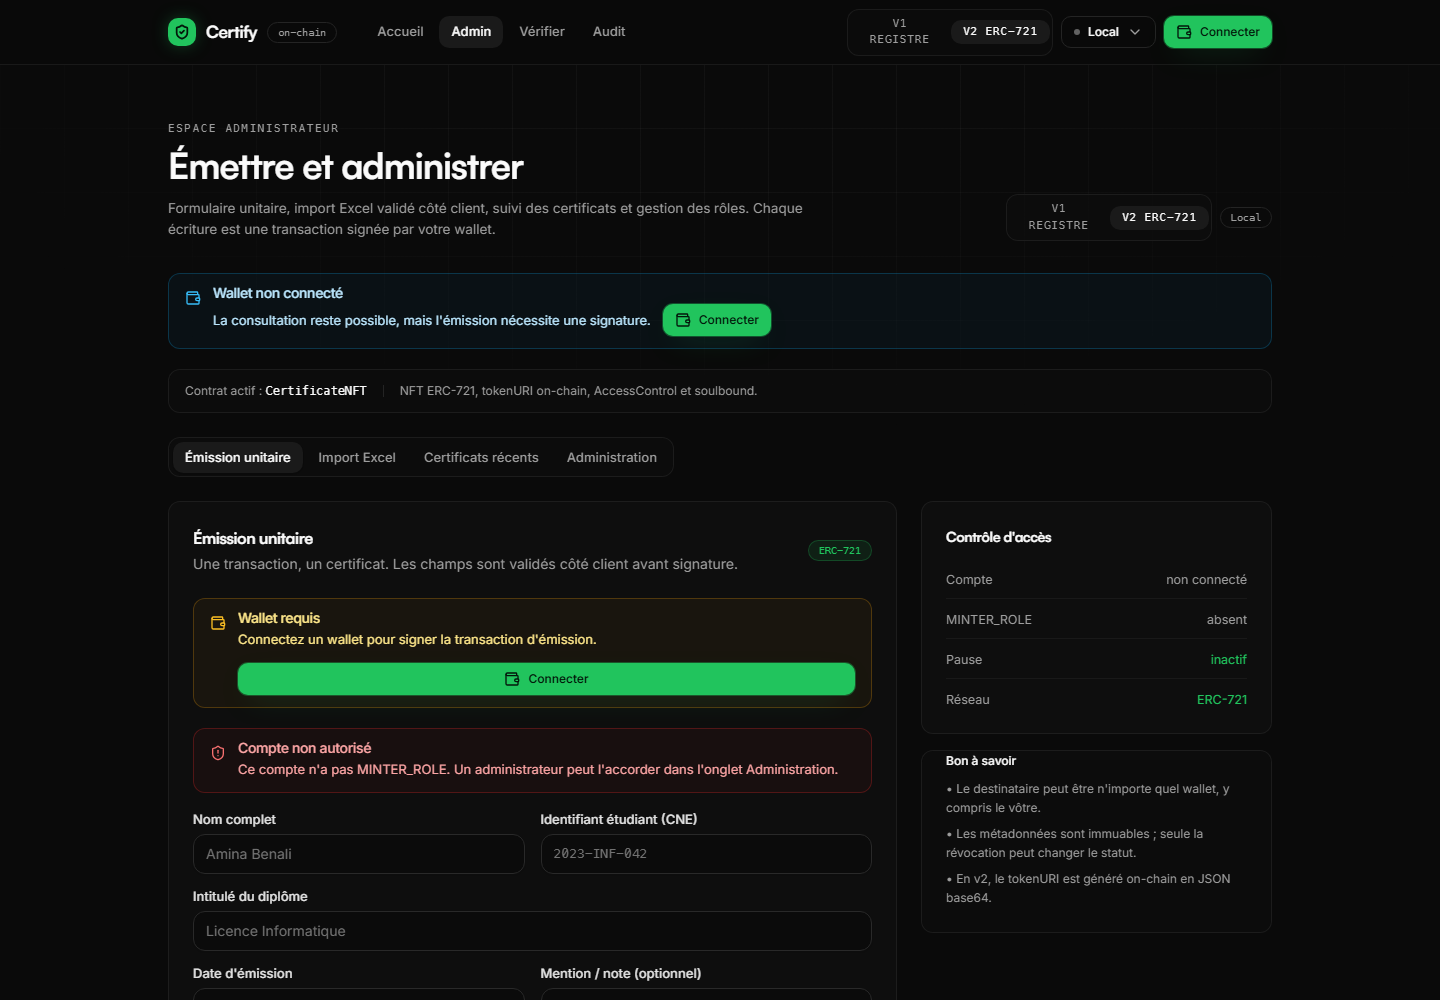
\includegraphics[width=0.92\textwidth]{02-admin.png}
\caption{Émission dans l'onglet \texttt{v1 · registre}.}
\label{fig:admin}
\end{figure}

\begin{figure}[htbp]
\centering
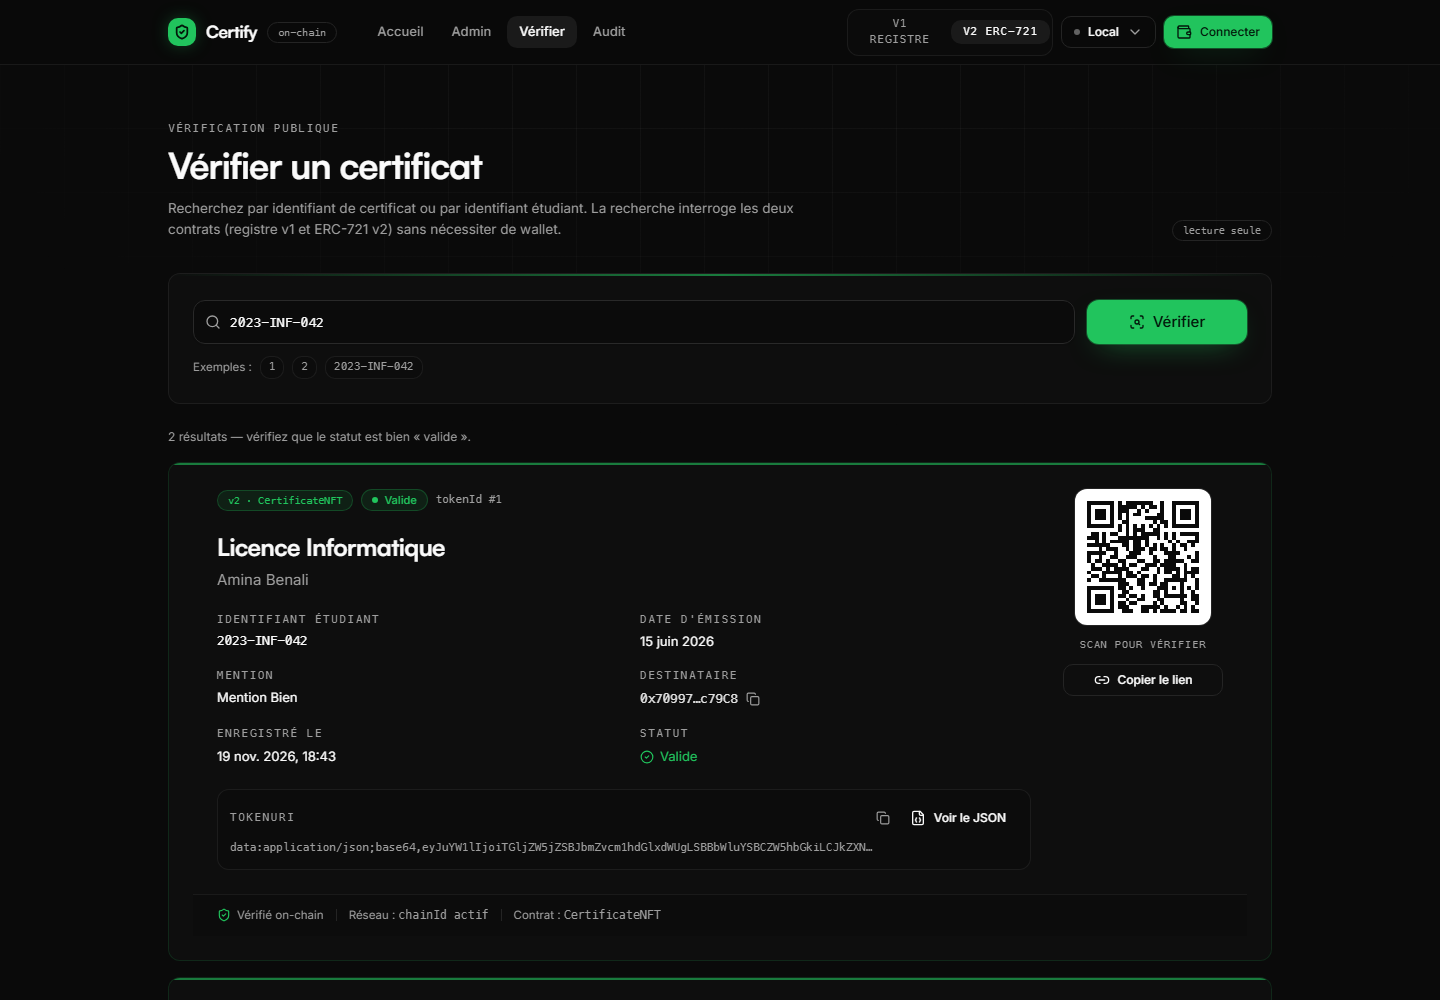
\includegraphics[width=0.92\textwidth]{04-verify-student.png}
\caption{Vérification publique de \texttt{2023-INF-042}.}
\label{fig:verify}
\end{figure}

La connexion passe par un wallet injecté. Sans extension MetaMask dans le
navigateur, wagmi renvoie \texttt{Provider not found} ; le bouton teste
maintenant les connecteurs disponibles et affiche un message explicite avant
d'appeler \texttt{connect()}. La vérification publique, elle, fonctionne sans
wallet puisqu'elle lit directement le RPC.

\section{Ce qui reste ouvert}

\begin{itemize}
\item Les chaînes ne sont pas bornées on-chain : un émetteur pourrait envoyer
  des textes très longs et faire monter le coût du gas.
\item La normalisation du \texttt{studentId} en majuscules est faite côté client.
  Un appel direct au contrat pourrait créer deux variantes d'un même identifiant.
\item Slither et le fuzzing Foundry n'ont pas été lancés ici. Le rapport d'audit
  du Devoir 2 reprend ces points plus en détail.
\item Aucun déploiement Sepolia n'est validé dans ce livrable ; les scripts sont
  prêts, la référence reste le réseau local.
\end{itemize}

\section{Pour relancer}

\begin{lstlisting}[basicstyle=\ttfamily\small]
cd certificats
npm install
npm run node           # terminal 1
npm run deploy:local   # terminal 2
npm run seed:local
npm run dev            # terminal 3
\end{lstlisting}

\end{document}
